\chapter{Automatizált Internet mérő rendszer}
(13-15 oldal): 


\section{Mérési elrendezés}
(5 oldal): traceroute, iperf, mérési forgatókönyvek, PlanetLab

\subsection{A PlanetLab hálózata}

A PlanetLab konzorcium egyetemi, ipari és kormányzati intézmények együttműködő csoportja, amelyek együttműködése fejleszti és támogatja a PlanetLab számítógépes hálózatot. A résztvevő szervezetek megosztják saját erőforrásaikat és hozzáférnek a hálózatba kötött számítógépekhez. Ilyen módon a résztvevők kivételes lehetőséghez jutnak, hogy  nagyméretű hálózatokon és elosztott rendszereken tudjanak vizsgálatokat végezni.

A konzorciumot 2002-ben alapította 10 amerikai egyetem az Intel Research közreműködésével, kezdetben 100 számítógép-csomópont létrehozásával. A közösségi teszthálózat évről évre bővült újabb egyetemek és ipari kapcsolatok csatlakozásával. A PlanetLab 2004-ben több Amerikán kívüli szervezetet is befogadott többek között európából, brazíliából és ázsiából. Ebben az évben így már világméretűvé nőtt és több mint 400 számítógép csomóponttal rendelkezett. Napjainkban ez a szám már túllépte az ezret és az \ref{fig:planetlab} ábrán látható, hogy a föld minden táján megtalálhatóak a hálózatban résztvevő csomópontok.

\begin{figure}[!ht]
	\centering
	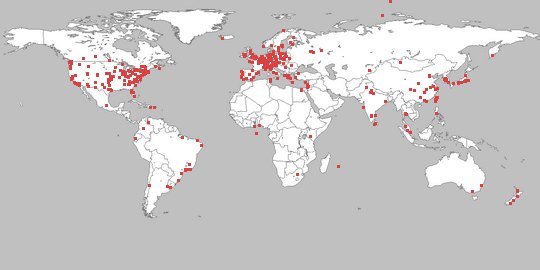
\includegraphics[width=0.65\textwidth, keepaspectratio]{figures/planetlab_worldmap.png}
	\caption{A PlanetLab teszthálózat csomópontjainak elhelyezkedése a világtérképen\label{fig:planetlab}}
\end{figure}

\subsection{Csatlakozás a hálózat számítógépeihez}

A tervezett mérések elvégzéséhez szükséges volt a csomópontokhoz való automatizált csatlakozás és parancs végrehajtás. Ehhez a PlanetLab központi szervere szolgált egyszerűen lekérhető listát a hálózatban résztvevő csomópontok címéről. A mérések elvégzéséhez és feldolgozásához egységesen Python programozási nyelven megírt szkripteket használtam. A méréseket végző 
program a Paramiko\cite{paramiko} könyvtárat használja az ssh kapcsolatok felépítéséhez és menedzseléséhez. A mérési kísérletek sok esetben hiúsultak meg különböző hibák miatt, vagy a célszámítógép elérhetetlensége miatt, ezért ezen esetek kezelése fontos szempont volt a fejlesztés során. Az \ref{fig:statistics} ábrákon látható statisztikák a márciusi mérések adataiból készültek. A mérések óránként lettek elvégezve, lefutásonként 1354 csomóponthoz téve csatlakozási kísérletet. A vezérlő számítógép nem állandóan futott, így a hónapban csak 23 nap készültek mérések, átlagosan 15 alkalommal.

\subsection{Időzített mérési forgatókönyvek}
Az iperf mérések implementálásakor több új eljárás kidolgozására volt szükség a mérést menedzselő szoftverben. A korábbi traceroute mérések egyetlen parancs távoli futtatásából álltak, amelyek futási eredményét tároltuk el mérési eredményként. Az iperf és más sávszélesség mérő szoftverek működéséhez azonban szükséges mind egy adatcsomagokat küldő és egy adatcsomagokat fogadó példány futtatása a két különböző távoli gépen. Ennek lebonyolításához a mérést lebonyolító programnak több szálon kell futnia, a két távoli kódfuttatást egyszerre kell végeznie. Először az adatcsomagok fogadását (szerver oldal) végző programot kell elindítani, majd csak ezt követően lehet csak a mérést megkezdeni az adatcsomagokat küldő program (kliens oldal) elindításával. A mérést követően a szervert pedig le kell állítani. Ez a szituáció tovább bonyolódik, ha két sávszélesség mérést párhuzamosan szeretnénk végezni. Ez egy fennálló igény, mivel a későbbiekben az MPTCP\footnote{Multipath Transfer Protocol: Több párhuzamos TCP adatfolyamon végez kommunikációt a felsőbb rétegek felé egyetlen TCP kapcsolatot emulálva.} protokoll lehetséges viselkedését is vizsgálni szeretnénk.

Ezeket a lépéseket általánosítva olyan mérési forgatókönyvek létrehozását támogatja már a mérési rendszer, amely bármilyen távoli parancsok időzített futtatását garantálja. Ennek kialakítása a lehető legrugalmasabbra lett tervezve, amelynek működését a függelékben található példakód mutatja be. A kód egyszerűségének ellenére a mérés teljesen menedzselt, bármilyen hiba keletkezése le van kezelve és megfelelően naplózva és a mérési eredményben jelezve van. Garantálva van a helyes időzítés, a párhuzamos futás és a helyes leállás.

A mérési forgatókönyvek rendkívül hasznos eszközzé váltak, a segítségükkel új mérések implementálása kényelmes és gyors.